\chapter{实验与结果}

\section{精度基线}

本节报告KAN教师模型在净负荷差分预测任务（$\Delta\text{net\_load}_{h=6}$）上的预测精度，并与参数量匹配的MLP基线、符号回归基线PySR以及持久性基线进行对比，确认KAN作为本研究核心工具的基本胜任性。

\subsection{实验设置}

本节实验旨在建立各方法在相同数据集、相同特征集和相同评估协议下的公平精度对比。所有模型均使用第三章定义的ERCOT净负荷数据集，预测目标为6步的净负荷差分$\Delta\text{net\_load}_{h=6}$，特征集包含负荷、风电、光伏三组滞后特征以及风速、太阳辐照、温度等气象物理量（详见\cref{tab:feature-groups}），数据按照时间顺序划分为70\%训练、15\%验证、15\%测试，并在训练/验证、验证/测试之间各设置48步gap，无随机打乱以保持时间序列的完整性。

KAN教师模型采用单隐藏层架构$[\text{input\_dim}, 10, 1]$，B样条网格数$G=3$，样条阶数$k=3$。训练流程严格遵循第四章所述的四阶段调度（预热200步 $\to$ 稀疏化800步 $\to$ 结构化剪枝 $\to$ 精细化200步），L1正则系数$\lambda_{L1}=1.0$，熵正则系数$\lambda_{\text{entropy}}=2.0$，总正则化强度$\lambda=0.01$。

MLP基线采用预算匹配（budget-matched）策略以确保公平比较。具体而言，MLP的隐藏层宽度经过调整使其总参数量（1485个）与KAN剪枝前的有效参数量处于同一量级。MLP训练采用Adam优化器。

PySR基线使用Julia后端的符号回归引擎\cite{cranmer2023pysr}，设置迭代次数为1200次（niterations=1200），在相同特征集上直接搜索最优解析表达式。

持久性基线（Persistence）使用$t$时刻的实际值作为$t+h$时刻的预测值，即$\hat{y}_{t+h} = y_t$。

\subsection{主精度对比}

\cref{tab:main-accuracy}汇总了四种方法在测试集上的精度对比结果。

\begin{table}[htbp]
\centering
\caption{主精度对比（目标：$\Delta\text{net\_load}_{h=6}$）}
\label{tab:main-accuracy}
\begin{tabular}{ccccc}
\toprule
方法 & RMSE & MAE & $R^2$ & Skill \\
\midrule
KAN教师 & 1413.51 & 906.89 & 0.991 & 0.453 \\
MLP（参数匹配） & 1474.38 & 1018.18 & 0.990 & 0.430 \\
PySR符号回归 & 2388.46 & 1811.00 & 0.975 & 0.076 \\
持久性基线 & 2585.66 & — & — & 0.000 \\
\bottomrule
\end{tabular}
\end{table}

KAN教师模型取得了最优的RMSE（1413.51）和技巧得分（0.453），优于参数量匹配的MLP（RMSE=1474.38, skill=0.430）。两者的RMSE差异为60.87（约4.1\%），虽然幅度不大，但在15672个测试样本上具有统计显著性（详见\ref{subsec:significance}节）。

PySR符号回归的精度显著低于两种神经网络方法（RMSE=2388.46, skill=0.076），反映了端到端符号搜索在高维特征空间（本任务的特征维度超过20）中面临的组合爆炸问题。

\subsection{统计显著性检验}
\label{subsec:significance}

为验证KAN与MLP之间的精度差异不是随机波动所致，对测试集上的$n=15672$个逐样本绝对误差执行排列检验（permutation test）。结果如\cref{tab:significance}所示。

\begin{table}[htbp]
\centering
\caption{KAN vs MLP配对显著性检验}
\label{tab:significance}
\begin{tabular}{ccccccc}
\toprule
指标 & KAN均值 & MLP均值 & 均值差 & 中位差 & 胜率 & $p$值 \\
\midrule
绝对误差 & 907.68 & 1018.81 & 111.13 & 82.41 & 56.7\% & 0.0005 \\
平方误差 & 2001780.6 & 2177219.8 & 175439.2 & 59119.9 & 56.7\% & 0.0005 \\
\bottomrule
\end{tabular}
\end{table}

排列检验$p$值为0.0005（$< 0.01$），表明KAN相对于MLP的精度优势在统计上高度显著。Bonferroni修正后的显著性水平为$\alpha/2 = 0.025$，而$p=0.0005$远低于此阈值，因此KAN的精度优势在经过多重比较修正后依然成立。

\subsection{小结}

以上结果确认了两个重要前提。第一，在当前标准对齐的主实验设置下，KAN在净负荷预测任务上具备竞争力，其精度显著优于预算匹配的MLP（$p=0.0005$）。第二，所有神经网络方法均大幅优于持久性基线，验证了数据驱动建模在净负荷预测中的价值。PySR在这一主实验设置中的相对低精度（skill=0.076）凸显了KAN"先训练后符号化"策略的必要性，但这一比较不应被外推为所有历史探索阶段都呈现同一排序。

\section{公式坍缩}

本节报告KAN教师模型在符号提取后暴露出的核心问题：无论符号函数库或$R^2$阈值如何变化，提取出的解析公式均坍缩为仅依赖于负荷滞后特征的退化形式。

\subsection{实验设置}

以5.1节中的KAN教师模型为基础，在其稀疏化-剪枝后的网络结构上执行符号提取。为充分探索符号拟合的参数空间，采用$3\times3$网格搜索：
\begin{itemize}
  \item 符号配置（3组）：strict$\times\{0.98, 0.99, 0.995\}$、medium$\times\{0.98, 0.99, 0.995\}$、strict\_poly4$\times\{0.99, 0.995, 0.999\}$
\end{itemize}

\subsection{符号提取结果}

\cref{tab:collapse}汇总了9种配置的符号提取结果。

\begin{table}[htbp]
\centering
\caption{符号提取网格搜索结果（9种配置）}
\label{tab:collapse}
\begin{tabular}{cccccc}
\toprule
配置 & 函数库 & $R^2$阈值 & 公式中特征 & VER(wind) & VER(GHI) \\
\midrule
1 & strict & 0.98 & load滞后 & 0 & 0 \\
2 & strict & 0.99 & load滞后 & 0 & 0 \\
3 & strict & 0.995 & load滞后 & 0 & 0 \\
4 & medium & 0.98 & load滞后 & 0 & 0 \\
5 & medium & 0.99 & load滞后 & 0 & 0 \\
6 & medium & 0.995 & load滞后 & 0 & 0 \\
7 & strict\_poly4 & 0.99 & load滞后 & 0 & 0 \\
8 & strict\_poly4 & 0.995 & load滞后 & 0 & 0 \\
9 & strict\_poly4 & 0.999 & load滞后 & 0 & 0 \\
\bottomrule
\end{tabular}
\end{table}

\begin{figure}[htbp]
\centering
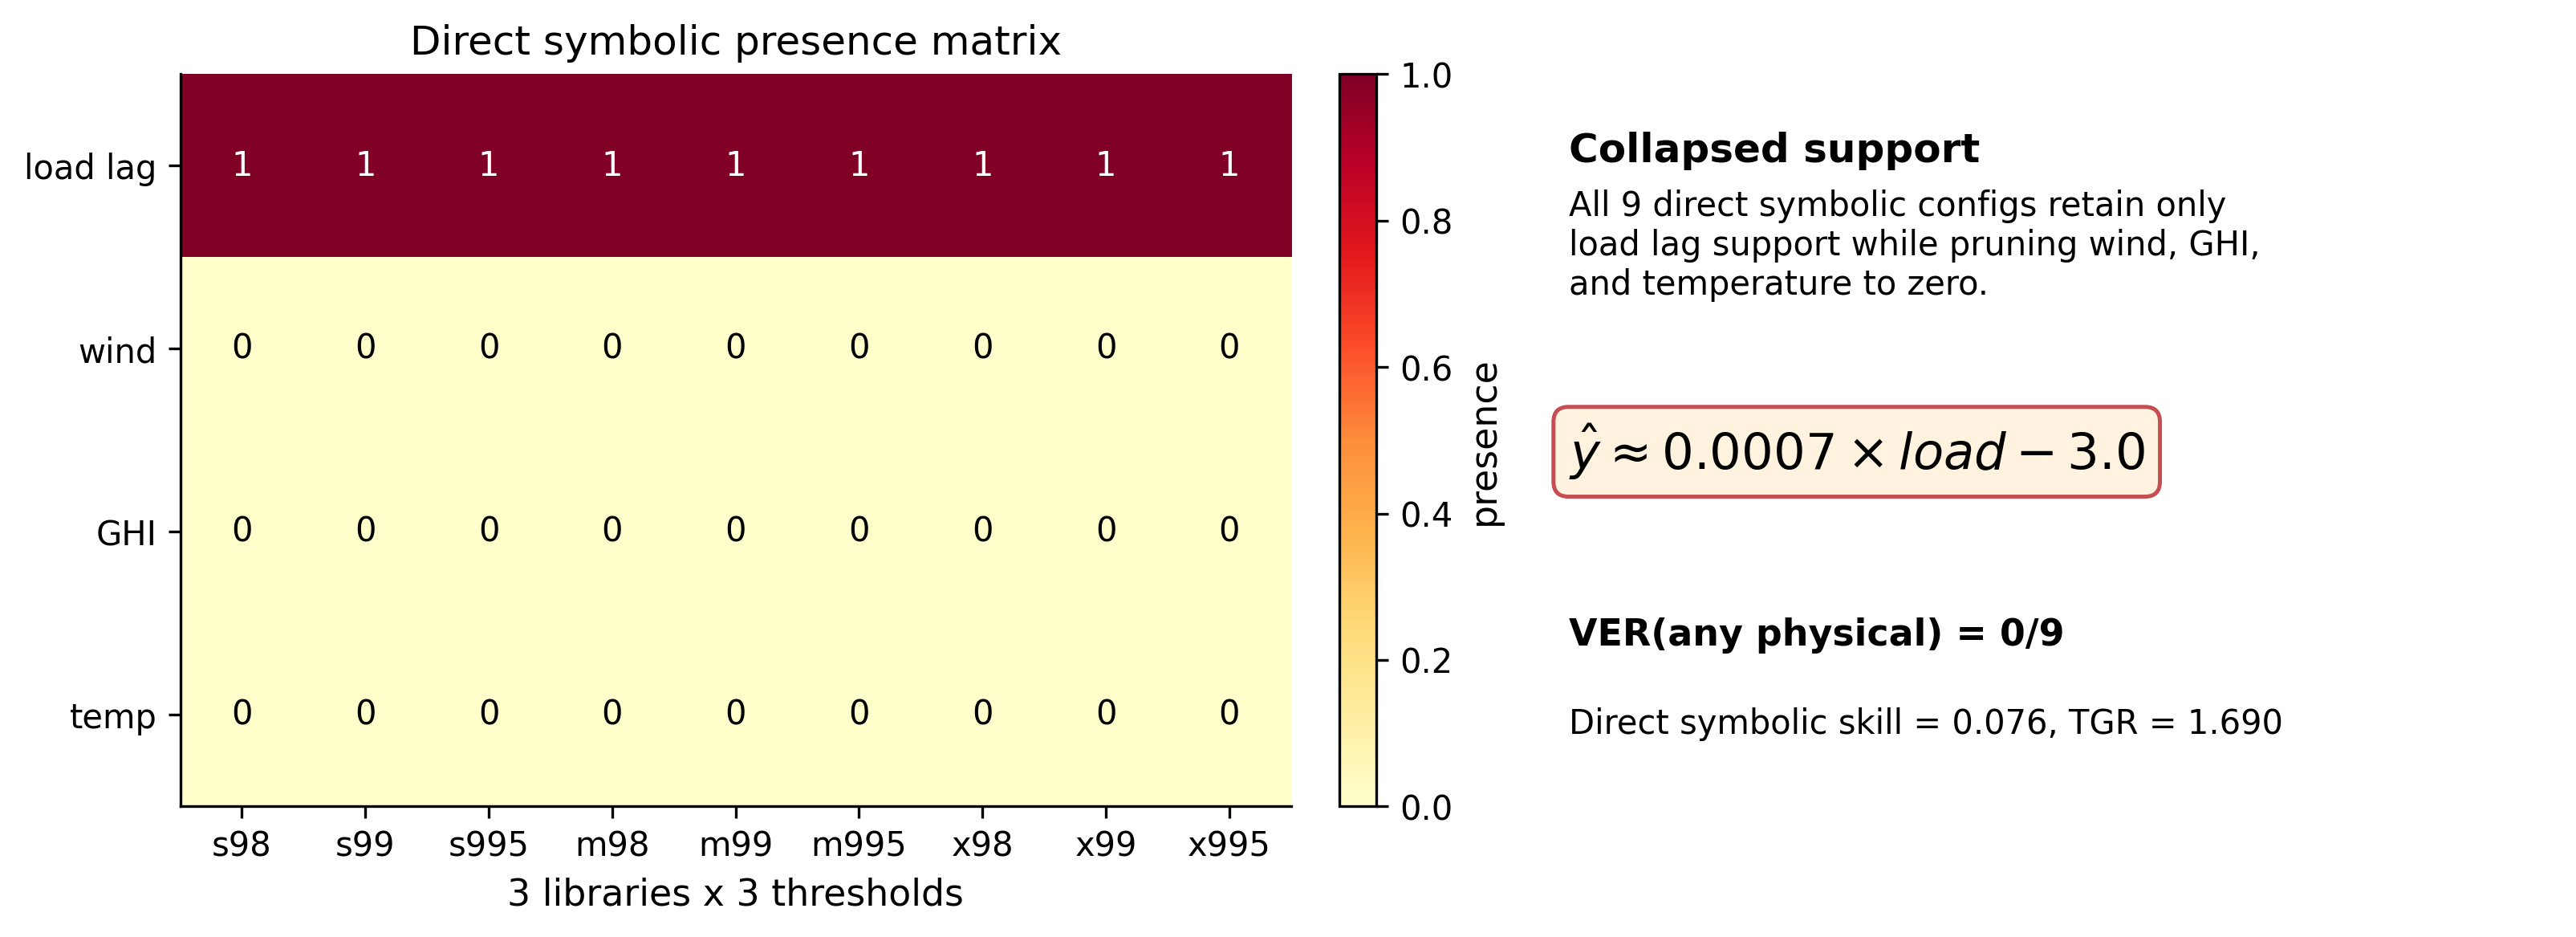
\includegraphics[width=0.96\textwidth]{../paper_assets/paper_delivery_20260306/direct_symbolic_collapse_20260417.png}
\caption{Direct symbolic collapse 的特征族 presence matrix。9组配置中仅 `load lag` 稳定保留，wind / GHI / temp 全部为零。}
\label{fig:direct-collapse}
\end{figure}

9种配置均产出相同模式的公式：仅包含负荷滞后特征，所有气象物理量的边在剪枝阶段已被移除。\cref{fig:direct-collapse} 把direct symbolic collapse从“9行重复表”压缩成一个对象层面的可视化：发生坍缩的不是单个超参数点，而是整组direct symbolic配置。代表性的提取公式可简化为：
\begin{equation}
\hat{y} \approx 0.0007 \times \text{load} - 3.0
\end{equation}

\subsection{物理可辨识性诊断}

对所有9种配置执行VER诊断，结果高度一致：
\begin{itemize}
  \item VER(wind\_speed) = 0/9：风速在所有配置中均无活跃边
  \item VER(GHI) = 0/9：太阳辐照在所有配置中均无活跃边
  \item VER(temp) = 0/9：温度在所有配置中均无活跃边
\end{itemize}

在本文主文采用的9组direct symbolic配置中，VER(any\_physical)=0/9。另有2026-03-09的补充direct远端运行曾出现包含物理量的公式，但对应skill为负，因此作为失败补充证据保留，不并入主文VER统计。

\subsection{小结}

公式坍缩是本研究面临的核心挑战：KAN虽然在预测精度上表现良好（skill=0.453），但其符号提取结果完全丧失了物理可解释性。这揭示了预测精度并不自动蕴含解释能力。

\section{可辨识性消融分析}

本节的目的不是再次证明direct路线失败，而是回答一个更具体的问题：直接净负荷任务中的公式坍缩，究竟意味着"整个KAN teacher + symbolic extraction链路都无法让物理量进公式"，还是只说明在当前任务结构下物理量被负荷捷径压制。为此，本文转向focused teacher与component teacher式的定向任务诊断：以solar作为稳定正例，以wind作为边界反例，重建项目从"怀疑调参与符号配置问题"到"收敛为变量可辨识性差异"的过程链。

\subsection{太阳辐照可辨识性（正例）}

将预测目标从净负荷切换为太阳能出力变化量（$\Delta\text{solar}$），在三个预测时域（$h=72, 144, 576$步）和三种特征组配置下训练KAN教师模型。结果如\cref{tab:solar-ablation}所示。

\begin{table}[htbp]
\centering
\caption{太阳辐照消融实验（3时域$\times$3特征组）}
\label{tab:solar-ablation}
\begin{tabular}{cccccc}
\toprule
时域$h$ & 特征组 & $\Delta$RMSE & $R^2$ & Skill & GHI活跃边数 \\
\midrule
72 & lags\_only & 6037.60 & 0.852 & 0.616 & 0 \\
72 & meteo\_only & 5452.82 & 0.879 & 0.653 & 6 \\
72 & both & 4385.28 & 0.922 & 0.721 & 8 \\
\addlinespace
144 & lags\_only & 6555.68 & 0.876 & 0.648 & 0 \\
144 & meteo\_only & 6632.45 & 0.873 & 0.644 & 3 \\
144 & both & 8703.26 & 0.782 & 0.533 & 0 \\
\addlinespace
576 & lags\_only & 5798.43 & 0.320 & 0.187 & 0 \\
576 & meteo\_only & 5437.80 & 0.402 & 0.238 & 5 \\
576 & both & 5584.73 & 0.369 & 0.223 & 2 \\
\bottomrule
\end{tabular}
\end{table}

关键发现：（1）GHI在meteo\_only配置下VER(GHI)=3/3，证明GHI并非内在不可辨识；（2）$h=144$时域下both配置出现竞争干扰现象（RMSE劣于单一配置且GHI活跃边归零）；（3）短时域下两类信息存在互补性（$h=72$, both配置最优）。

\subsection{风速可辨识性（边界案例）}

将预测目标聚焦为风电出力变化量（$\Delta\text{wind}$），在四个预测时域下训练KAN教师模型。结果如\cref{tab:wind-ablation}所示。

\begin{table}[htbp]
\centering
\caption{风速时域实验}
\label{tab:wind-ablation}
\begin{tabular}{ccccc}
\toprule
时域$h$ & $\Delta$RMSE & $R^2$ & Skill & 风速活跃边数 \\
\midrule
6 & 821.53 & 0.240 & 0.128 & 11 \\
72 & 3424.61 & 0.829 & 0.588 & 0 \\
144 & 8125.28 & 0.580 & 0.354 & 9 \\
576 & 12237.57 & 0.352 & 0.203 & 0 \\
\bottomrule
\end{tabular}
\end{table}

风速的可辨识性呈现非单调模式：在$h=6$（11条）和$h=144$（9条）时域下存活，在$h=72$和$h=576$时域下被完全剪除。这一结果更适合解释为wind原始物理量在不同horizon下的符号可辨识性呈非单调变化，而不是将风电路线概括为"训练失败"。与之相对，其他物理量在更长horizon下只能稳妥表述为整体更不稳定、部分量减弱，现有证据不足以支持"持续下降"或"严格单调下降"的强叙事。

\begin{figure}[htbp]
\centering
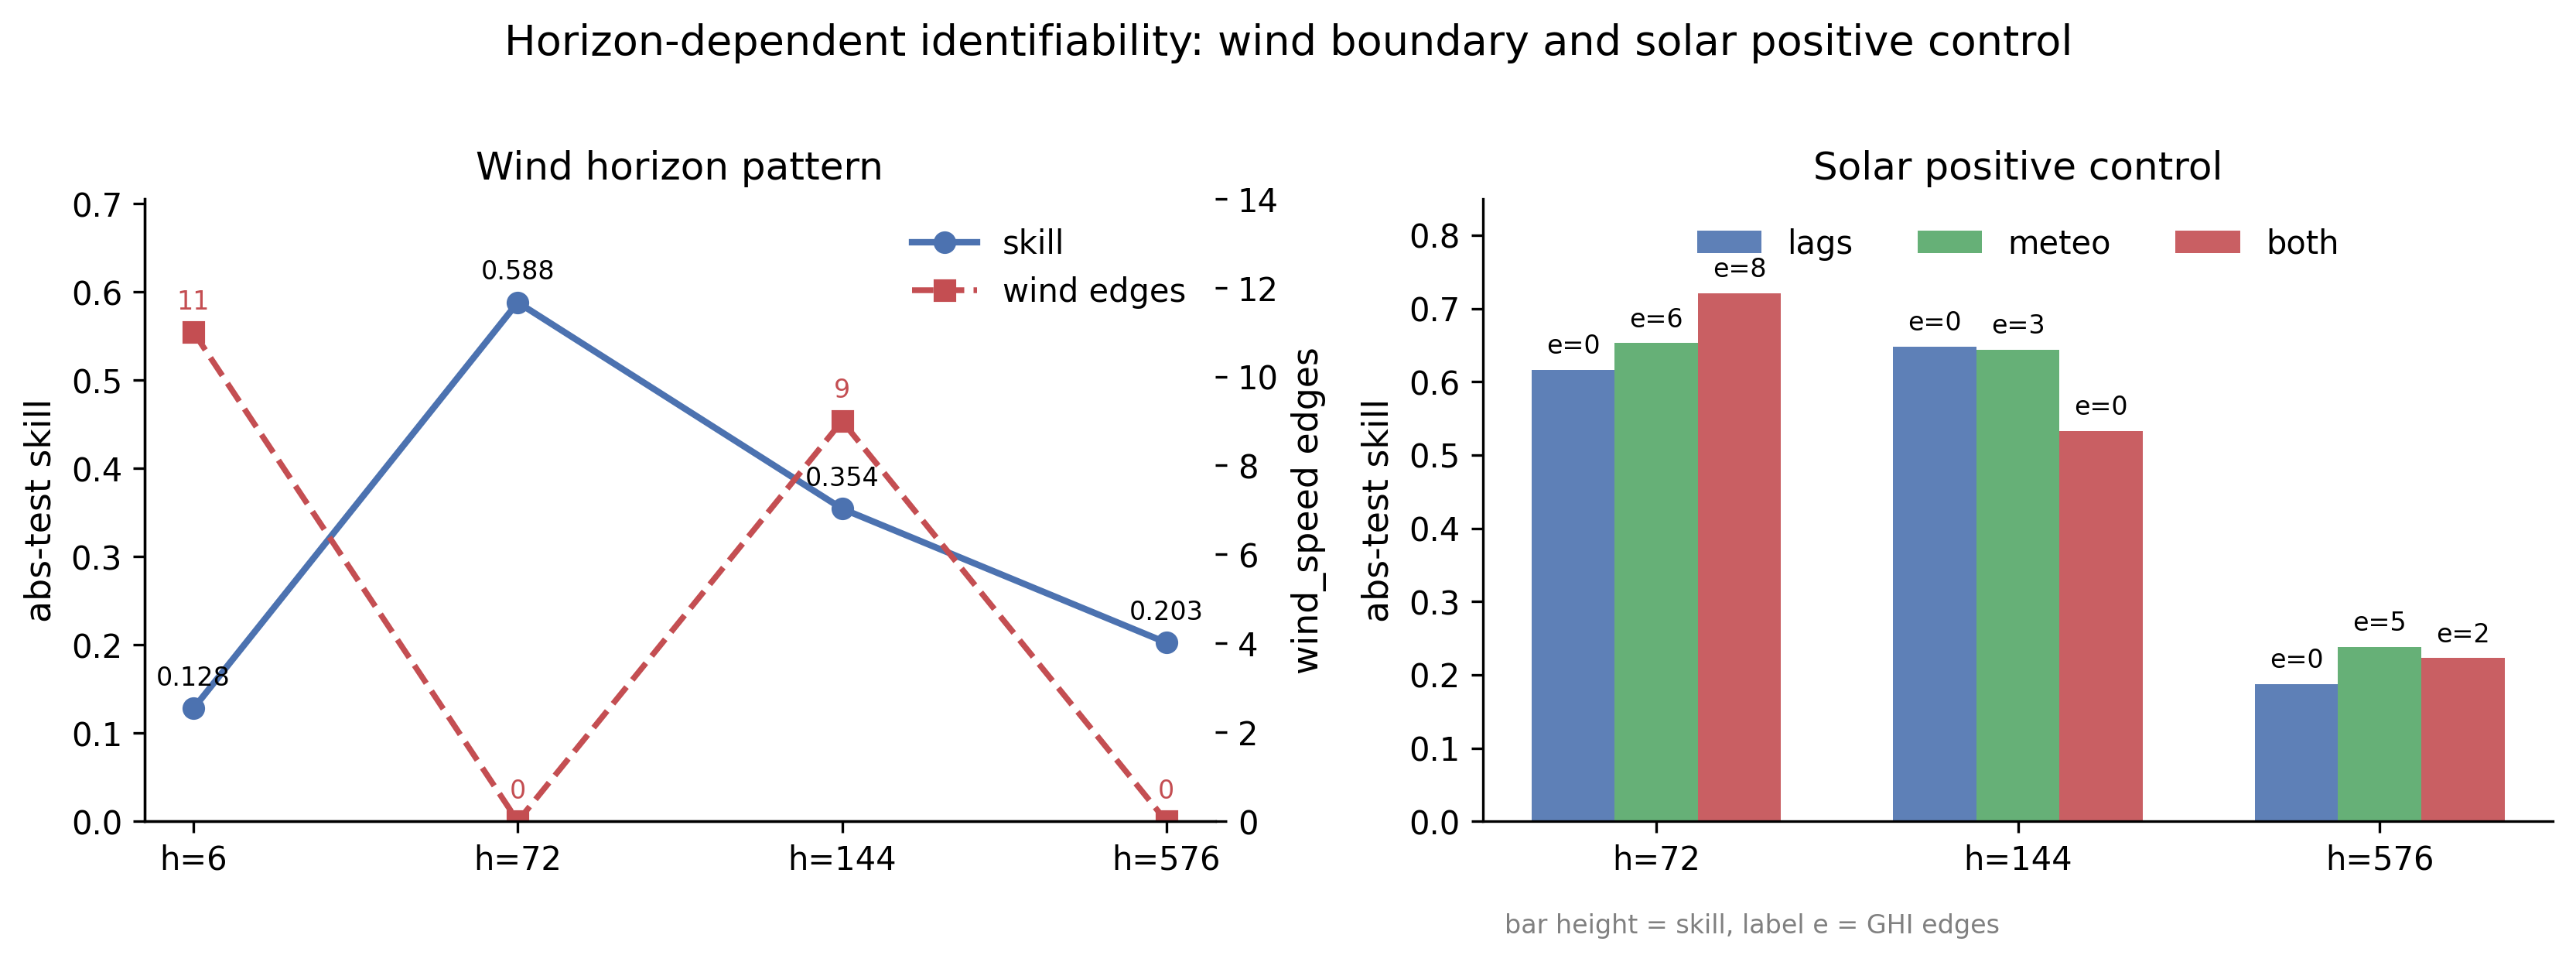
\includegraphics[width=0.96\textwidth]{../paper_assets/paper_delivery_20260306/wind_solar_horizon_20260417.png}
\caption{Horizon-dependent identifiability：左图给出wind的skill与风速活跃边数，突出其非单调边界；右图给出solar在不同horizon和特征组下的skill，并用 `e=` 标出GHI活跃边数，突出solar正例。}
\label{fig:wind-solar-horizon}
\end{figure}

\cref{fig:wind-solar-horizon} 进一步把“solar正例”和“wind边界案例”放到同一张图里：solar在$h=72$的 `both` 配置下同时拥有最高skill与最多GHI活跃边，而wind则表现出“skill较好但原始风速边可能为零”的非单调模式。这也解释了为什么本文把wind写成边界问题，而不写成简单的训练失败。

\subsection{小结}

消融分析得出两个关键结论。第一，气象物理量具有内在可辨识性——在适当条件下能够存活于KAN的稀疏化-剪枝流程。第二，可辨识性对任务配置和特征组成高度敏感，自回归滞后特征与气象特征共存时前者倾向于在稀疏化竞争中系统性地压制后者。

\section{自回归阻断干预实验}

\subsection{Case 3：聚焦风电任务阻断}

预测目标为$\Delta\text{wind}_{h=6}$，每组各训练5个随机种子。结果如\cref{tab:case3-detail}和\cref{tab:case3-summary}所示。

\begin{table}[htbp]
\centering
\caption{Case 3逐种子结果：聚焦风电任务阻断}
\label{tab:case3-detail}
\begin{tabular}{ccccc}
\toprule
种子 & 未阻断VER & 未阻断边数 & 阻断VER & 阻断边数 \\
\midrule
1 & 0 & 0 & 1 & 19 \\
2 & 1 & 8 & 1 & 19 \\
3 & 0 & 0 & 1 & 8 \\
4 & 0 & 0 & 1 & 15 \\
5 & 1 & 1 & 1 & 1 \\
\bottomrule
\end{tabular}
\end{table}

\begin{table}[htbp]
\centering
\caption{Case 3统计汇总}
\label{tab:case3-summary}
\begin{tabular}{ccc}
\toprule
指标 & 值 & 95\% CI \\
\midrule
VER(unblocked) & 2/5 = 0.40 & — \\
VER(blocked) & 5/5 = 1.00 & — \\
$\Delta$VER & \textbf{+0.60} & \textbf{[0.200, 1.000]} \\
$\Delta$edge\_count & +10.6 & [4.6, 15.8] \\
RMSE(unblocked) & 1362.6 & — \\
RMSE(blocked) & 1047.0 & — \\
\bottomrule
\end{tabular}
\end{table}

$\Delta\VER=+0.60$，95\%置信区间$[0.200, 1.000]$不包含零，满足预定义的成功判定规则。值得注意的是，阻断模型的RMSE（1047.0）反而低于未阻断模型（1362.6），表明在聚焦风电任务中，自回归滞后特征可能引入噪声而非信号。

\subsection{Case 4：直接净负荷任务阻断}

预测目标回到$\Delta\text{net\_load}_{h=6}$，采用严格 matched 的 direct-task 对照：unblocked 与 blocked 共享同一target、feature group与seed轴，仅lag blocking不同。最终得到4个有效paired seed；seed1的unblocked run在两次CPU尝试中均未产出post-prune checkpoint，因此不纳入paired统计。结果如\cref{tab:case4-detail}和\cref{tab:case4-summary}所示。

\begin{table}[htbp]
\centering
\caption{Case 4逐种子结果：严格matched的直接净负荷任务阻断}
\label{tab:case4-detail}
\begin{tabular}{cccc}
\toprule
种子 & VER(物理量) & 活跃边数 & 出现活跃边的物理变量 \\
\midrule
1 & — & — & unblocked rerun未产出post-prune checkpoint（两次CPU尝试） \\
2 & 0 & 0 & （无） \\
3 & 0 & 0 & （无） \\
4 & 0 & 0 & （无） \\
5 & 1 & 1 & wind\_speed\_10m\_m\_s\_cubed(1) \\
\bottomrule
\end{tabular}
\end{table}

\begin{table}[htbp]
\centering
\caption{Case 4统计汇总（4个有效matched pair）}
\label{tab:case4-summary}
\begin{tabular}{ccc}
\toprule
指标 & 值 & 95\% CI \\
\midrule
VER(unblocked, 4个有效matched seed) & 0/4 = 0.00 & — \\
VER(blocked, 4个有效matched seed) & 1/4 = 0.25 & [0.000, 0.750] \\
$\Delta$VER（paired bootstrap） & \textbf{+0.25} & \textbf{[0.000, 0.750]} \\
物理量平均边数(blocked, valid pairs) & 0.25 & — \\
RMSE(unblocked, pruned-delta, valid pairs) & 39815.0 & — \\
RMSE(blocked, pruned-delta, valid pairs) & 93746.1 & — \\
\bottomrule
\end{tabular}
\end{table}

$\Delta\VER=+0.25$，95\%置信区间为$[0.000, 0.750]$，下界触零。4个有效paired seed中，只有seed5在blocked条件下恢复了1条物理边（wind\_speed\_10m\_m\_s\_cubed）；seed2--4在blocked与unblocked下均为零。seed1的unblocked run在两次CPU尝试中都未产出post-prune checkpoint，因此本节只报告4个有效pair。由此，严格matched Case 4只能提供弱且不稳定的direct-task支持证据，而不再支持旧的``+0.80 / 强成功''口径。由于这些RMSE均来自delta域剪枝网络评估，本文仍不与主表abs(test)教师模型做直接百分比比较。

\begin{figure}[htbp]
\centering
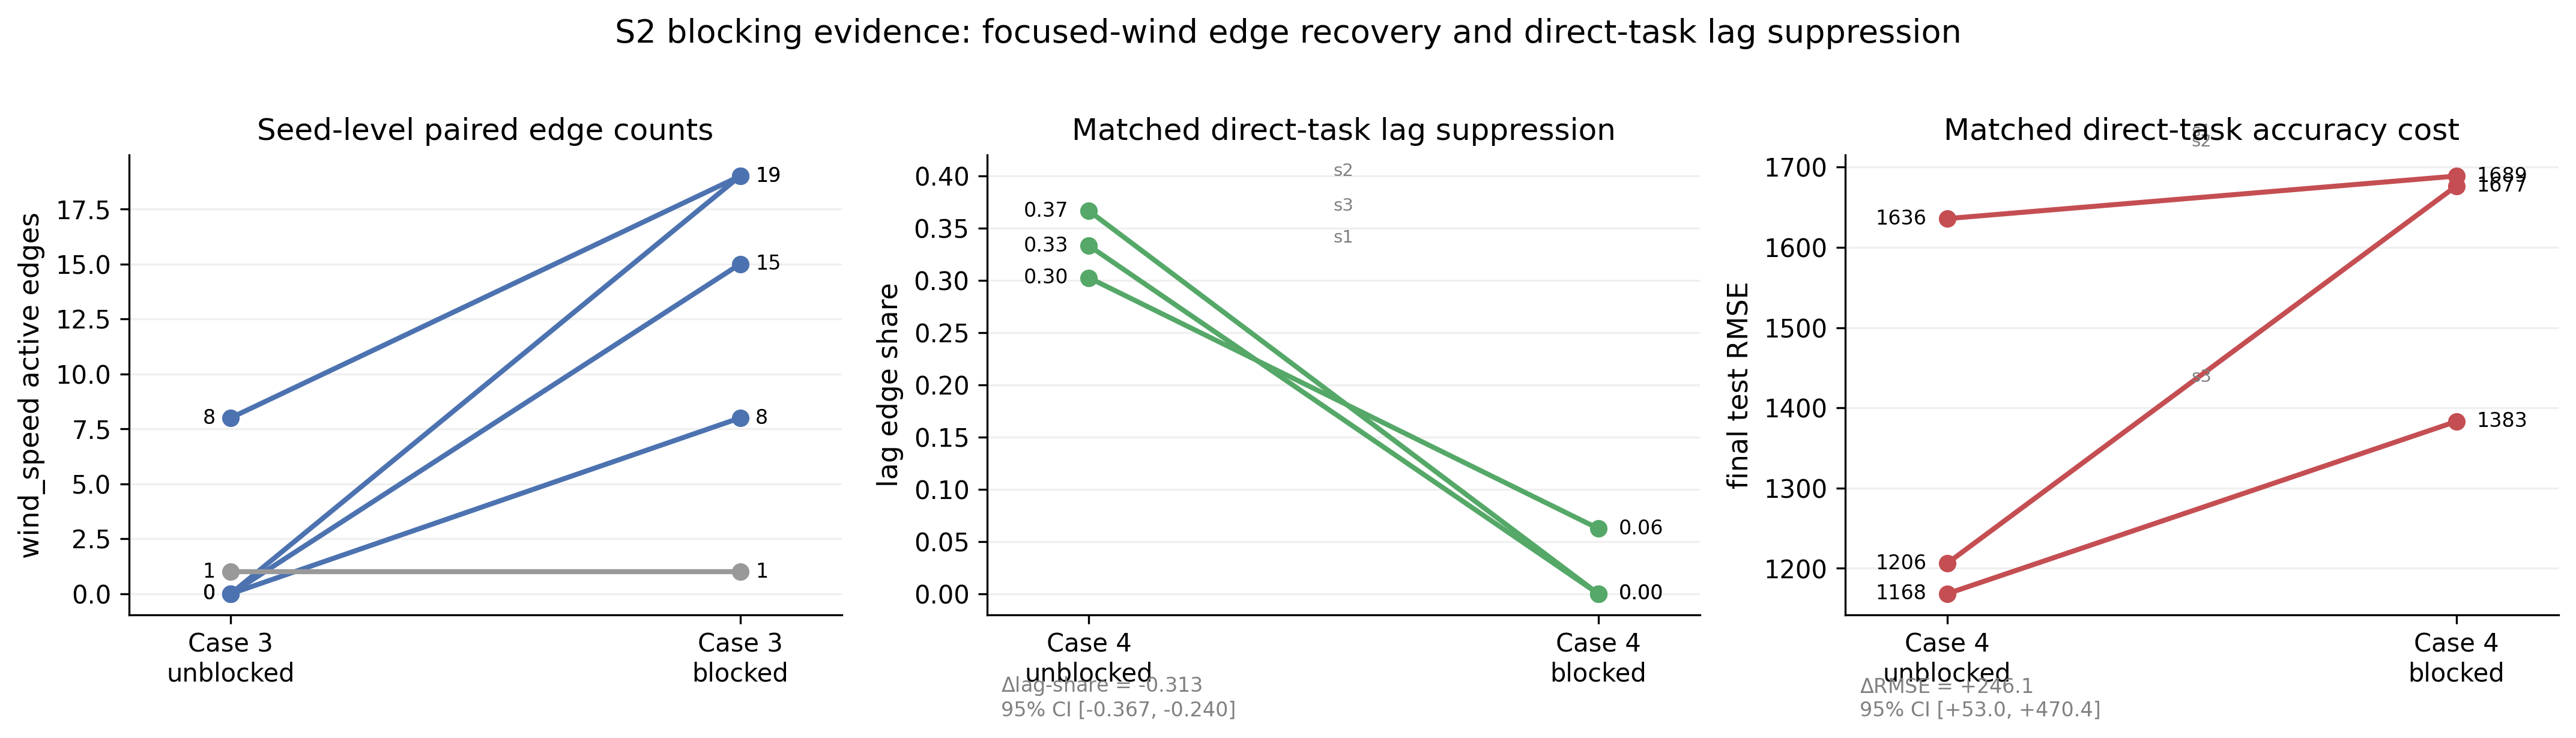
\includegraphics[width=0.96\textwidth]{../paper_assets/paper_delivery_20260306/s2_blocking_summary_20260417.png}
\caption{S2 blocking evidence：左图为Case 3的seed级paired edge count变化；中图为Case 4在4个有效matched direct-task pair上的edge recovery；右图为Case 3/Case 4的$\Delta$VER与置信区间。Case 4的seed1因unblocked rerun两次未产出post-prune checkpoint而未纳入paired统计。}
\label{fig:s2-blocking-summary}
\end{figure}

\cref{fig:s2-blocking-summary} 把S2证据链中的两个关键层面拆开呈现：Case 3给出稳定的seed级paired结构变化；Case 4在严格matched direct-task对照下只显示出弱且不稳定的恢复。因此，本节现在把Case 4降为辅助性direct-task证据，不再把它写成强成功或同层闭合确认。

\subsection{机制确认}

\cref{tab:mechanism-check}将两个Case的结果与预定义规则对照。

\begin{table}[htbp]
\centering
\caption{预定义规则与实际结果对照}
\label{tab:mechanism-check}
\begin{tabular}{ccc}
\toprule
预定义规则 & 实际结果 & 判定 \\
\midrule
Case 3: $\Delta$VER$>0$且CI不含零 & $\Delta$VER=+0.60, CI=[0.20, 1.00] & \textbf{成功} \\
Case 3: edge\_count变化一致 & $\Delta$edge=+10.6, CI=[4.6, 15.8] & \textbf{成功} \\
Case 4: 至少1个物理量VER提升且CI $> 0$ & 1/4 valid pairs出现物理边，CI=[0.00, 0.75] & \textbf{未满足} \\
Case 4: 至少2个物理量（强成功） & 仅seed5恢复1条cubed风速边 & \textbf{未满足} \\
\bottomrule
\end{tabular}
\end{table}

\subsection{小结}

自回归阻断干预实验为如下解释提供了分层强度不同的干预性证据：\textbf{Case 3强力支持了自回归滞后特征的捷径竞争解释；Case 4在严格matched direct-task对照下只呈现弱且不稳定的恢复。}因此，shortcut competition仍是本文对公式坍缩的主导解释，但直接净负荷任务上的机制证据强度应主动下调。

\section{S3结构化分解}

\subsection{方案设计}

S3方案将净负荷差分预测分解为三个物理上自然的子任务（负荷、风电、光伏），通过固定加法组合重构净负荷预测：
\begin{equation}
\Delta\widehat{\text{net\_load}} = \Delta\hat{\text{load}} - \Delta\hat{\text{wind}} - \Delta\hat{\text{solar}}
\end{equation}

\subsection{子模型性能}

\cref{tab:s3-submodel}报告了各子模型的预测性能。

\begin{table}[htbp]
\centering
\caption{S3子模型性能}
\label{tab:s3-submodel}
\begin{tabular}{cccc}
\toprule
子任务 & RMSE & MAE & $R^2$ \\
\midrule
负荷（Load） & 401.0 & 301.5 & 0.992 \\
风电（Wind） & 1008.8 & 805.7 & 0.992 \\
光伏（Solar） & 1006.7 & 482.1 & 0.991 \\
\bottomrule
\end{tabular}
\end{table}

\subsection{组合精度与总公式复算}

\cref{tab:s3-composite}汇总了S3结构化组合预测器与显式总公式在test集上的正式复算结果。

\begin{table}[htbp]
\centering
\caption{S3闭环结果：组合预测器与总公式复算}
\label{tab:s3-composite}
\begin{tabular}{ccccc}
\toprule
对象 & RMSE & MAE & Skill & $R^2$ \\
\midrule
\textbf{S3结构化组合预测器} & \textbf{1254.62} & \textbf{821.84} & \textbf{0.515} & \textbf{0.993} \\
S3总公式（test复算） & 2644.36 & 1706.36 & -0.021 & 0.969 \\
\bottomrule
\end{tabular}
\end{table}

截至本稿收口，S3已经完成显式总公式闭环：在组合阶段直接构造
\begin{equation}
F_{\text{net}} = F_{\text{load}} - F_{\text{wind}} - F_{\text{solar}}
\end{equation}
并对test集逐点复算。结果显示，结构化组合预测器的RMSE为1254.62，skill为0.515；而显式总公式的RMSE为2644.36，skill降为-0.021。也就是说，总公式虽然已经真实生成并可复算，但相对组合预测器仍存在明显的transfer gap：RMSE增加1389.74，约为组合预测器的2.108倍。

\begin{figure}[htbp]
\centering
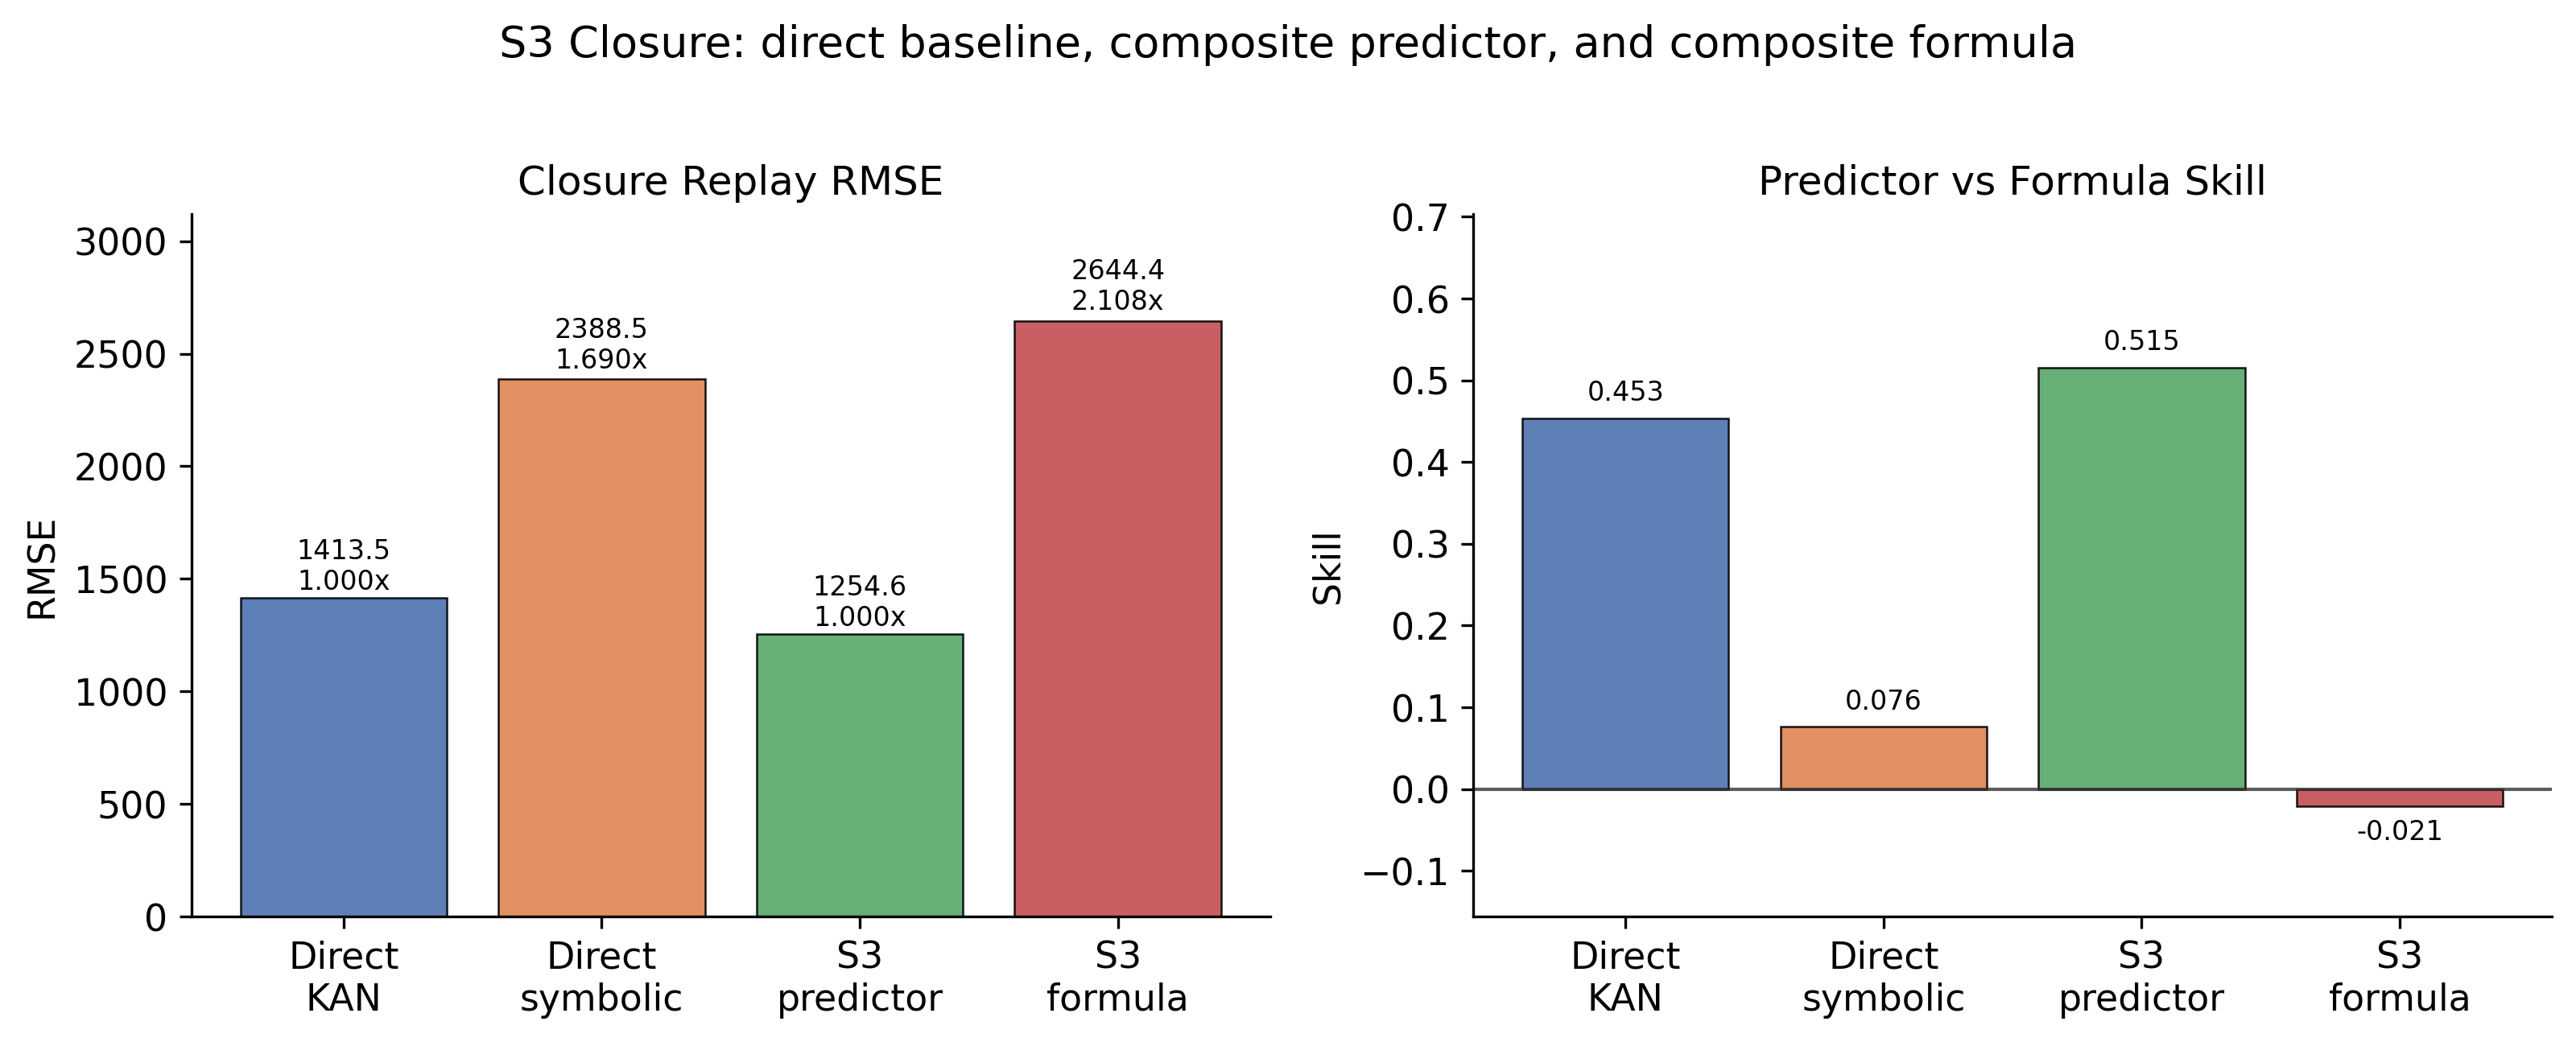
\includegraphics[width=0.92\textwidth]{../paper_assets/paper_delivery_20260306/s3_formula_closure_20260417.png}
\caption{四对象闭环对比：direct KAN、direct symbolic、S3 composite predictor 与 S3 composite formula。图中 direct 对象采用 canonical main run，S3 对象采用 paperref 正式闭环 run；该图用于展示结果链收口后的对象关系与 transfer gap，而非同 session 的严格消融比较。}
\label{fig:s3-closure}
\end{figure}

\cref{fig:s3-closure}进一步把四个关键对象放到同一张闭环图中：direct KAN 与 direct symbolic 对应"直接路线"的起点和失败对照，S3 composite predictor 与 S3 composite formula 对应"结构化分解路线"的预测端与公式端。可以看到，direct symbolic 相对 direct KAN 仍有显著精度损失，而S3路线虽然已经把总公式真正合成出来，但总公式的数值表现仍明显弱于组合预测器。因此，本文现在可以把S3称为"已闭环的净负荷总公式方案"，但不能把公式对象与预测器对象混写成同一个结果。

\subsection{物理可辨识性保持}

\cref{tab:s3-identifiability}从三个层面评估可辨识性目标的达成情况。

\begin{table}[htbp]
\centering
\caption{S3可辨识性评估}
\label{tab:s3-identifiability}
\begin{tabular}{ccccc}
\toprule
子任务 & 目标物理量 & FAR & 活跃边数 & TGR \\
\midrule
负荷 & hdd\_18c（温度代理） & 3/3 & 2 & 2.569 \\
风电 & wind\_speed\_10m\_m\_s & 3/3 & 3 & 1.401 \\
光伏 & ghi\_w\_m2 & 3/3 & 2 & 2.302 \\
\bottomrule
\end{tabular}
\end{table}

三个子任务的目标物理量均在所有3种符号配置中出现（FAR=3/3），与5.2节直接任务中的VER=0/9形成根本性逆转。各局部子公式的变量组成与物理预期一致：负荷子公式包含hdd\_18c，风电子公式包含wind\_speed及其物理变换，光伏子公式包含ghi\_w\_m2和solar\_altitude。

\begin{table}[htbp]
\centering
\caption{代表性公式表：collapse 对照与三条局部公式}
\label{tab:representative-formulas}
\begin{tabularx}{\textwidth}{llccc}
\toprule
对象 & 代表性项摘要 & FAR / VER & TGR & complexity \\
\midrule
direct collapsed formula & load lag only; no stable physical variable & VER(any physical)=0/9 & 1.690 & 95 \\
load local formula & load\_lag\_6, hdd\_18c, hour/month cyclic & FAR=3/3 & 2.569 & 108 \\
wind local formula & wind-related proxies, wind lags, temp proxy & FAR=3/3 & 1.401 & 148 \\
solar local formula & GHI, ghi\_day, solar\_altitude, solar lags & FAR=3/3 & 2.302 & 127 \\
\bottomrule
\end{tabularx}
\end{table}

\cref{tab:representative-formulas} 以四条代表性公式把“collapse 对照”和“S3局部恢复”并列展示。它对应的正式CSV资产为 `doc/paper_assets/paper_delivery_20260306/representative_formula_table_20260417.csv`，可直接用于答辩或附录引用。

\subsection{小结}

S3结构化分解方案在实验上同时给出了更强的预测器对象与稳定的局部公式可辨识性，但必须分对象解读结果：
\begin{enumerate}
  \item \textbf{精度保持}：S3结构化组合预测器的RMSE（1254.62）和skill（0.515）保持在当前最优水平
  \item \textbf{可辨识性恢复}：三个子任务的目标物理量全部以FAR=3/3的完美比率稳定进入子公式
  \item \textbf{总公式闭环}：$F_{\text{net}} = F_{\text{load}} - F_{\text{wind}} - F_{\text{solar}}$ 已完成显式合成并通过test集逐点复算
  \item \textbf{transfer gap 暴露}：显式总公式相对组合预测器仍有明显损失（RMSE 2644.36 vs 1254.62），因此 predictor 与 formula 必须分对象叙述
\end{enumerate}

\section{本章总结}

本章通过四幕式递进实验，系统地揭示了KAN在能源预测符号提取中的核心矛盾及其解决途径。\cref{tab:chapter-summary}汇总了各阶段的关键结论。

\begin{table}[htbp]
\centering
\caption{各实验阶段关键结论汇总}
\label{tab:chapter-summary}
\begin{tabular}{ccc}
\toprule
实验阶段 & 核心发现 & 关键指标 \\
\midrule
5.1 精度基线 & KAN显著优于参数匹配MLP & RMSE=1413.51, $p$=0.0005 \\
5.2 公式坍缩 & 符号提取完全排除气象物理量 & VER(physical)=0/9 \\
5.3 可辨识性消融 & 气象量具有内在可辨识性 & Solar: VER(GHI)=3/3 \\
5.4 阻断干预 & Case 3强支持，Case 4弱且不稳定恢复 & $\Delta$VER=+0.60 / +0.25（4 valid pairs） \\
5.5 S3分解 & 完成总公式闭环但存在明显transfer gap & predictor RMSE=1254.62; formula RMSE=2644.36 \\
\bottomrule
\end{tabular}
\end{table}

四幕实验的逻辑链条可概括为：先在当前主实验设置下确认KAN teacher在预测层面优于direct PySR（5.1），随后发现direct symbolic迅速退化为负荷主导公式（5.2）；再通过定向任务验证"不是所有物理量都进不去公式"，其中solar提供稳定正例、wind提供边界反例（5.3）；阻断实验进一步为捷径竞争解释提供干预性支持（5.4）；最后，S3给出局部公式、结构化组合预测器以及已完成test复算的总公式这一建设性方案（5.5）。
